\section*{Specific Aims}

The goal of this research is to develop an optical system for simultaneous imaging of neural activity using calcium and voltage indicators. 
The common practice in brain imaging is to use two photon (2P) excitation,  combined with sequential scanning of the brain volume. However, this scanning reduces frame rate; moreover, it offers an inefficient  use of imaging time, as we are  interested in monitoring specific spatially distributed groups of neurons and not the entire brain.
To allow reading neural activity at a high frame rate we aim to
use a holographic illumination pattern targeted at a neural population of interest, and simultaneously measure their activity using a 2D sensor. 
 Even when using 2P excitation, the emitted light  undergoes significant scattering and existing  holographic recording systems cannot see beyond $200\mu m$ of tissue.
 To overcome aberrations caused by tissue scattering we plan to incorporate spatial light modulators (SLM) for wavefront shaping. 
 %both the  excitation wavefronts as well as the outgoing emitted ones. 

The project will involve two parallel aims. The first one corrects the emission of 2P systems, and the second one uses single-photon (1P) excitation systems. Since 1P systems involve shorter wavelengths the incoming illumination is also scattered  and we  have to correct it. 
While 2P excitation suffer  from reduced scattering, it requires very high powers, and as a result heat and safety considerations imply that no more than $10-20$ neurons can be simultaneously excited.  
On the other hand, 1P excitation requires four orders of magnitude less power than 2P systems, thus we can excite a much larger group of neurons without heat concerns.
	\begin{figure*}[h!]\vspace{-0.2cm}
	\begin{center}
		\begin{tabular}{cccc}
			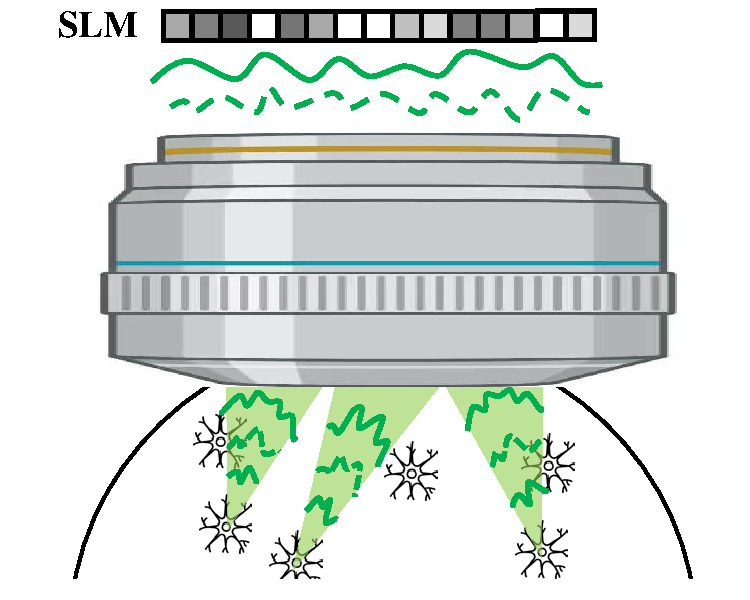
\includegraphics[width= 0.25\textwidth]{figs/timeline/illust.pdf}&&
		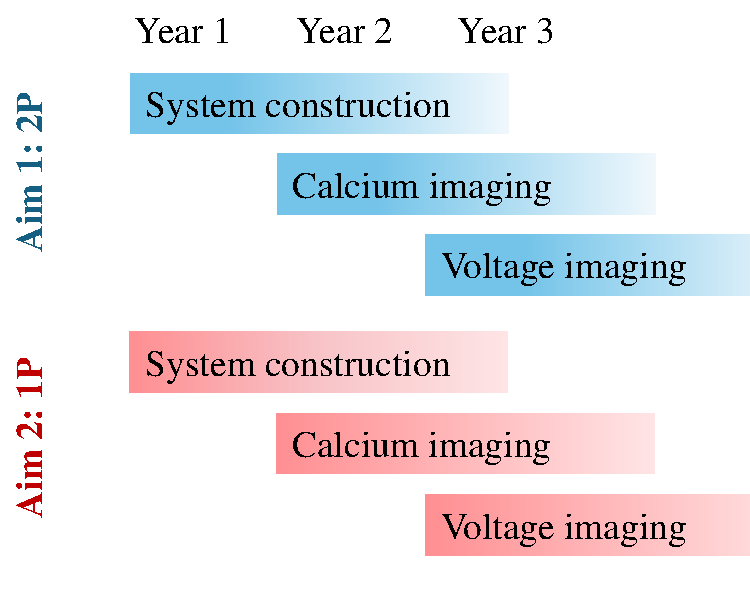
\includegraphics[width= 0.25\textwidth]{figs/timeline/timeline2.pdf}
		\end{tabular}\vspace{-0.6cm}
	\end{center}
	\caption{Left: Schematic for targeted neural recording with aberration correction. Right: Project timeline.\Anat{I read somewhere on the instructions that images are not allowed on the specific aims file, but on the other hand they ask for this timeline chart.}  } 
\vspace{-0.5cm}
\label{fig:timeline}
\end{figure*}


	\Anat{I am not sure the millstones and aims here are specific enough. This is the part I hate most in any proposal I write. Will appreciate help. To be honest I have no idea what depth we can actually image and I gave a very rough numbers hoping they are realistic. $\times 10$ SNR improvement I am rather confident we can achieve based on what I have seen in my lab, probably even more. Increasing the neurons density with 1P I also think should be easy}
We plan to work on both aims in parallel. Each track involves the following milestones. i) Year 1: system construction and alignment,  testing with ex-vivo   slices. ii) Year 2: in-vivo experiments with calcium indicators. iii)Year 3: in vivo experiments with voltage indicators, were both high frame and high SNRs are needed. iv) In parallel to the in-vivo experiments, in year 2 and 3 we will also further improved the algorithms beyond our system, increasing its noise robustness and accelerating its run-time.    We use the following evaluation metrics in all 3 stages. 


	
	\boldstart{Aim 1: correcting outgoing wavefronts in 2P excitation.}
For the $200\mu m$ depths considered in previous work using a standard 2D sensor, our correction can yield a $\times 10$ improvement in SNR. Moreover, our correction would allow pushing the depth of measurable neurons up to $500\mu m$.
	
	
	\boldstart{Aim 2: correcting outgoing and incoming wavefronts in 1P excitation.}
	 We will push the depth where 1P imaging is applicable and apply calcium imaging  $500-700\mu m$ deep into the tissue. Currently such depths are only accessible by expensive 2P lasers. 
	We will also apply the technique for voltage imaging and compare it against a one dimensional version (without fast scanning) of the targeted confocal voltage imaging work of~\cite{Xiao2024LargeScale}. We will show that for the $200-300\mu m$ depth range considered in their work, wavefront shaping can provide a $\times 10$ improvement in SNR.  We can also push the range of measurable depths to $500\mu m$. Compared to 2P excitation that cannot target more than $10-20$ neurons simultaneously, our 1P system will measure hundreds of neurons. 
